\documentclass[letterpaper,10pt]{article}

\usepackage{titling}
\usepackage{listings}
\usepackage{url}
\usepackage{setspace}
\usepackage{subfig}
\usepackage{sectsty}
\usepackage{pdfpages}
\usepackage{colortbl}
\usepackage{multirow}
\usepackage{relsize}
\usepackage{amsmath}
\usepackage{fancyvrb}
\usepackage{amsmath,amssymb,amsthm,graphicx,xspace}
\usepackage[titlenotnumbered,noend,noline]{algorithm2e}
\usepackage[compact]{titlesec}
\usepackage{paratype} 
\usepackage[T1]{fontenc}
\usepackage{tikz}
\usetikzlibrary{arrows,automata,shapes,trees,matrix,chains,scopes,positioning,calc}
\tikzstyle{block} = [rectangle, draw, fill=blue!20, 
    text width=2.5em, text centered, rounded corners, minimum height=2em]
\tikzstyle{bw} = [rectangle, draw, fill=blue!20, 
    text width=4em, text centered, rounded corners, minimum height=2em]

\definecolor{namerow}{cmyk}{.40,.40,.40,.40}
\definecolor{namecol}{cmyk}{.40,.40,.40,.40}

\let\LaTeXtitle\title
\renewcommand{\title}[1]{\LaTeXtitle{\textsf{#1}}}


\newcommand{\handout}[5]{
  \noindent
  \begin{center}
  \framebox{
    \vbox{
      \hbox to 5.78in { {\bf ECE254: Operating Systems and Systems Programming } \hfill #2 }
      \vspace{4mm}
      \hbox to 5.78in { {\Large \hfill #4  \hfill} }
      \vspace{2mm}
      \hbox to 5.78in { {\em #3 \hfill} }
    }
  }
  \end{center}
  \vspace*{4mm}
}

\newcommand{\lecture}[3]{\handout{#1}{#2}{#3}{Lecture #1}}
\newcommand{\tuple}[1]{\ensuremath{\left\langle #1 \right\rangle}\xspace}

\addtolength{\oddsidemargin}{-1.000in}
\addtolength{\evensidemargin}{-0.500in}
\addtolength{\textwidth}{2.0in}
\addtolength{\topmargin}{-1.000in}
\addtolength{\textheight}{1.75in}
\addtolength{\parskip}{\baselineskip}
\setlength{\parindent}{0in}
\renewcommand{\baselinestretch}{1.5}
\newcommand{\term}{Spring 2015}

\singlespace


\begin{document}

\lecture{ 22 ---  Caching }{\term}{Jeff Zarnett}

\section*{Caching}
\begin{quote}
\textit{Caching is very... hit and miss.}
\end{quote}


Caching is very important in computing, and not just memory. We examine the idea of caching in the context of memory, but it is applicable any time there is a large resource that is divided into pieces, some of which are used more often than others. The goal of caching is to speed up operations. It is desirable to read information from cache, when possible, because it takes less time to get data from cache to the CPU than from main memory to the CPU. CPUs are a lot faster than memory and it is best if we do not keep them waiting.

Caches do not have to operate on pages; they can operate on anything, but they are typically blocks of a given size. An entry in a cache is often called a \textit{line}. We will assume for the balance of this discussion that a cache line maps nicely to a page.

As discussed, the CPU generates a memory address for a read or write operation. The address will be mapped to a page. Ideally, the page is found in the cache, because that would be faster. If the requested page is, in fact,  in the cache, we call that a cache \textit{hit}. If the page is not found in the cache, it is considered a cache \textit{miss}. In case of a miss, we must load the page from memory, a comparatively slow operation. The percentage of the time that a page is found in the cache is called the \textit{hit ratio}, because it is how often we have a cache hit. We can calculate the effective access time if we have a good estimate of the hit ratio (which is not overly difficult to obtain) and some measurements of how long it takes to load data from the cache and how long from memory. The effective access time is therefore computed as:

\begin{center}
Effective Access Time = $h \times t_{c} + (1-h) \times t_{m}$
\end{center}

Where $h$ is the hit ratio, $t_{c}$ is the time required to load a page from cache, and $t_{m}$ is the time to load a page from memory. Of course, we would like the hit ratio to be as high as possible. 

Caches have limited size, because faster caches are more expensive. With infinite money we might put everything in registers, but that is rather unrealistic. Caches for memory are very often multileveled; Intel 64-bit CPUs tend to have L1, L2, and L3 caches. L1 is the smallest and L3 is the largest. See the diagram below:

\begin{center}
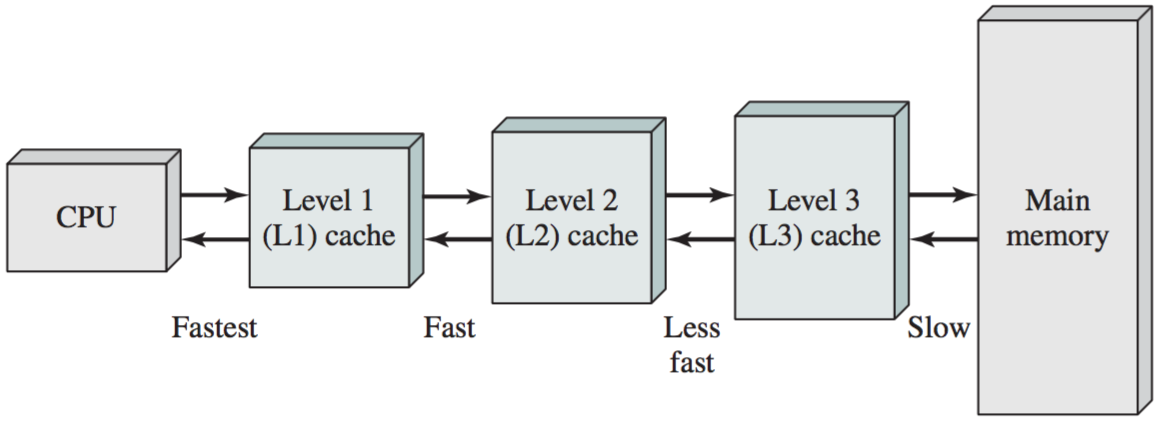
\includegraphics[width=0.6\textwidth]{images/caches.png}\\
Three levels of cache between the CPU and main memory~\cite{osi}.
\end{center}

If we have a miss in the L1 cache, the L2 cache is checked. If the L2 cache contains the desired page, it will be copied to the L1 cache and sent to the CPU. If it is not in L2, then L3 is checked. If it is not there either, it is in main memory and will be retrieved from there and copied to the in-between levels on its way to the CPU. Because caches have limited size, we have to manage this carefully.

\subsection*{Page Replacement Algorithms}
Whenever a page fault occurs, the operating system needs to choose which page to evict from the cache to make space for the new one. 

\bibliographystyle{alpha}
\bibliography{254}


\end{document}